\documentclass{beamer}

\usepackage{beamerthemesplit}
\usetheme{Singapore} %Copenhagen}
%\usecolortheme{whale}

%\usepackage[T2A]{fontenc}
%\usepackage[utf8]{inputenc}
%\usepackage[russian]{babel}

\usepackage[main=russian,english]{babel}   %% загружает пакет многоязыковой вёрстки
\usepackage{fontspec}      %% подготавливает загрузку шрифтов Open Type, True Type и др.
\defaultfontfeatures{Ligatures={TeX},Renderer=Basic}  %% свойства шрифтов по умолчанию
\setmainfont{Times New Roman} %% задаёт основной шрифт документа
%\usefonttheme{professionalfonts}% SOLUTION
\usefonttheme{serif}

\usepackage{hyperref}
\usepackage{textcomp}
\usepackage{amssymb,amsmath}
%\usepackage{animate}
%\usepackage{longtable}
\usepackage{xcolor}

%\usepackage{pgffor}
\usepackage{enumitem}
\usepackage[export]{adjustbox}

\newcounter{N}

%% Форматирование окружения itemize
%\usepackage{ragged2e}
%\let\olditem\item
%\renewcommand\item{\olditem\justifying}

\usepackage{ mathrsfs }
\newcommand{\Rho}{\mathscr{P}}

\renewcommand{\Re}{\operatorname{Re}}

\newcommand{\argxi}{(\xi^1,\xi^2,\xi^3)}
\newcommand{\argx}{(x^1,x^2,x^3)}

\newcommand{\argxiv}{(\vec{\xi})}
\newcommand{\argxv}{(\vec{x})}


\newcommand{\argxbarn}{(\bar{x}^1,\bar{x}^2,\ldots, \bar{x}^n)}
\newcommand{\argxn}{(x^1, x^2,\ldots, x^n)}

\newcommand{\argtxi}{(t, \xi^1,\xi^2,\xi^3)}
\newcommand{\argtoxi}{(t_0, \xi^1,\xi^2,\xi^3)}

\newcommand{\argtxiv}{(t, \vec{\xi})}
\newcommand{\argtoxiv}{(t_0, \vec{\xi})}


\newcommand{\argtx}{(t, x^1,x^2,x^3)}
\newcommand{\argtox}{(t_0, x^1,x^2,x^3)}

\newcommand{\argtxv}{(t, \vec{x})}
\newcommand{\argtoxv}{(t_0, \vec{x})}


\newcommand{\pd}[2]{\frac{\partial #1}{\partial #2}}
\newcommand{\pdk}[2]{\frac{\partial^2 #1}{\partial #2^2}}

\newcommand{\od}[2]{\frac{d #1}{d #2}}
\newcommand{\odk}[3]{\frac{d^{#3} #1}{d #2^{#3}}}

\newcommand{\grad}{\operatorname{grad}}
\newcommand{\rot}{\operatorname{rot}}
\newcommand{\divo}{\operatorname{div}}

\title[]{Движение твёрдого тела в идеальной жидкости}

\author[]{ {\em Верещагин Антон Сергеевич}
\\
канд. физ.-мат. наук, старший преподаватель\\
\bigskip
Кафедра аэрофизики и газовой динамики ФФ НГУ}

\usebackgroundtemplate{
\includegraphics[width=\paperwidth]{../img/background.png}}

\begin{document}
	
\frame{\titlepage}


\frame{
	\frametitle{Аннотация}
	\parbox{\textwidth}{
	Постановка задачи о движении тела в бесконечной идеальной жидкости, покоящейся на бесконечности. Степень убывания потенциала на бесконечности. Условие на поверхности тела и разложение Кирхгофа для потенциала. Гидродинамические реакции при движении тела. Импульсивная сила, пара. Коэффициенты присоединённой массы и их свойства.
	}
}

\frame{
	\frametitle{ Движение тела в безграничной жидкости }
	
		\begin{exampleblock}{Основная задача}
		\parbox{\textwidth}{
			Исследовать влияние бесконечной идеальной жидкости, покоящейся на бесконечности, на движение тела, ограниченного поверхностью $S$, имеющего поступательную скорость $\vec{U}$ и вращательную $\vec{\omega}$. Тело начинает движение из состояния покоя.
		}
	\end{exampleblock}
	
	\begin{columns}
		\begin{column}{0.5\textwidth}
			\centering
			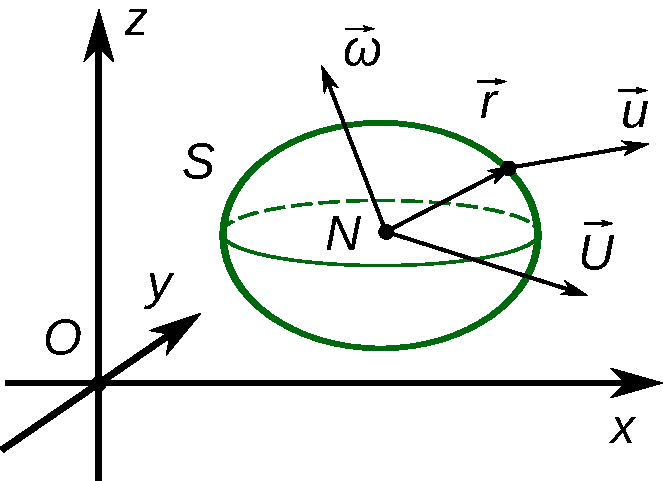
\includegraphics[width=\linewidth]{../img/body.pdf}
		\end{column}
		\begin{column}{0.5\textwidth}
			\begin{exampleblock}{Скорость движения точки тела}
				\parbox{\textwidth}{
				\[
					\vec{u} = \vec{U}+\vec{\omega}\times \vec{r}.
				\]	
				}
			\end{exampleblock}
			

		\end{column}
	\end{columns}


	
}

\frame{
	\frametitle{ Математическая постановка для жидкости}
	
	\begin{exampleblock}{Уравнение неразрывности }
		\parbox{\textwidth}{
			\[
			\pd{v_x}{x} + \pd{v_y}{y} + \pd{v_z}{z} = 0
			\]
			или по теореме Лагранжа для потенциальных течений
			\[
			\Delta \varphi = \pdk{\varphi}{x}+\pdk{\varphi}{y}+\pdk{\varphi}{z} = 0.
			\]
			
			
		}
	\end{exampleblock}
	\begin{exampleblock}{Условие на границе с телом}
		\parbox{\textwidth}{
			\[
			\pd{\varphi}{n} = u_n.
			\]
		}
	\end{exampleblock}

	\begin{exampleblock}{Условие на бесконечности}
		\parbox{\textwidth}{
			\[
			\lim\limits_{r\to\infty}\pd{\varphi}{x} = 
			\lim\limits_{r\to\infty}\pd{\varphi}{y} = 
			\lim\limits_{r\to\infty}\pd{\varphi}{z} = 0,\,
			\text{где}\,\,
			r = \sqrt{x^2+y^2+z^2}.
			\]

			
		}
	\end{exampleblock}
	
}

\frame{
	\frametitle{Распределение давление по пространству}
	
		\begin{exampleblock}{Интеграл Коши}
		\parbox{\textwidth}{
			\[
			\pd{\varphi}{t} + \frac{\nabla\varphi^2}{2} + \frac{p}{\rho} = f(t)\footnote{Считаем, что поле внешних сил отстутствует}
			\]
			
			Интеграл Коши позволяет найти распределение давления по заданному потенциалу, определённому из уравнения неразрывности ($\rho=const$).
		}
	\end{exampleblock}

	\begin{exampleblock}{Для бесконечно удалённой точки}
		\parbox{\textwidth}{
			\[
			p = p_0 - \rho\pd{\varphi}{t} - \frac{\rho v^2}{2},
			\]
			т.к. на бесконечности скорость жидкости равна $0$ а давление $p_0$.
		}
	\end{exampleblock}
}


\frame{
	\frametitle{Степень убывания потенциала на бесконечности}
	\begin{exampleblock}{Разложение потенциала по сферическим функциям}
		\parbox{\textwidth}{
			\[
			\varphi(r,\theta,\lambda) = \frac{A}{r}+\sum\limits_{n=1}^\infty\frac{Y_n(\theta,\lambda)}{r^{(n+1)}},
			\]
			где $Y_n(\theta,\lambda)$ -- сферические функции. Сферические функции и потенциал заданны в сферической системе координат.
			
		}
	\end{exampleblock} \pause
	\begin{exampleblock}{Уравнение неразрывности}
		\parbox{\textwidth}{
			Пусть $\Sigma$ -- сфера большого радиуса $R$ с центром в точке $O$, тогда
			\[
			\int_V\divo\vec{v} dV = \int_\Sigma \vec{v}\cdot\vec{n} dS =\int_\Sigma\pd{\varphi}{r}dS = 0
			\]
			или
			\[
			-4\pi A - \sum_{n=1}^\infty\frac{n+1}{R^{(n+2)}}\int_\Sigma Y_n(\theta,\lambda)dS = 0 \quad
			\overset{R\to\infty}{\Rightarrow}\quad
			A = 0.
			\]
		}
	\end{exampleblock}
}


\frame{
	\frametitle{Степень убывания потенциала на бесконечности}
	
	\begin{exampleblock}{Общий вид потенциала}
		\parbox{\textwidth}{
			\[
			\varphi(r,\theta,\lambda) = \sum\limits_{n=1}^\infty\frac{Y_n(\theta,\lambda)}{r^{n+1}}.
			\]
		}
	\end{exampleblock}

	\begin{exampleblock}{Вывод}
		\parbox{\textwidth}{
			Можно считать, что  $\displaystyle\pd{\varphi}{x}$, $\displaystyle\pd{\varphi}{y}$, $\displaystyle\pd{\varphi}{z}$ стремятся к $0$ при $r \to \infty $ как величины порядка \alert{$1/r^3$}, а $\varphi$ -- как \alert{$1/r^2$}.
			
		}
	\end{exampleblock}
	
}

\frame{
	\frametitle{Условие на поверхности тела}
	
	\begin{exampleblock}{Скорость точек тела}
		\parbox{\textwidth}{
			\[
			u_x = U_x + \omega_y z - \omega_z y,\quad
			u_y = U_y + \omega_z x - \omega_x z,\quad
			u_z = U_z + \omega_x y - \omega_y z.
			\]
		}
	\end{exampleblock}
	
	\begin{exampleblock}{Скорость точек на поверхности тела вдоль нормали}
		\parbox{\textwidth}{
			Обозначим 
			\[
			\cos(\widehat{n,x}) = \alpha,\quad
			\cos(\widehat{n,y}) = \beta,\quad
			\cos(\widehat{n,z}) = \gamma
			\]
			для косинусов углов, составляемых нормалью к поверхности $S$ с осями координат.
			
			\alert{Нормальная составляющая скорости} к поверхности $S$
			\[
			u_n = u_x\alpha + u_y\beta+ u_z\gamma = 
			(U_x + \omega_y z - \omega_z y)\alpha + 
			(U_y + \omega_z x - \omega_x z)\beta +
			\]
			\[
			+
			(U_z + \omega_x y - \omega_y z)\gamma.
			\]
		}
	\end{exampleblock}
	
}

\frame{
	\frametitle{Условие на поверхности тела}


	\begin{exampleblock}{Соотношение для потенциала}
		\parbox{\textwidth}{
			\[
			\left. \pd{\varphi}{n}\right|_S = U_x\alpha + U_y\beta + U_z\gamma + 
			\omega_x(y\gamma-z\beta) + \omega_y(z\alpha-x\gamma) + \omega_z (x\beta - y\alpha).
			\]
			
			Здесь $U_x$, $U_y$, $U_z$, $\omega_x$, $\omega_y$, $\omega_z$ -- функции от времени, а выражения справа от них --  функции точек пространства, формы поверхности $S$, координаты тела, а значит и времени.
			
		}
	\end{exampleblock}


}



\frame{
	\frametitle{ Условие на поверхности тела }
		\begin{exampleblock}{Вид потенциала в форме Кирхгофа}
		\parbox{\textwidth}{
			\[
			\varphi = U_x \varphi_1 + U_y \varphi_2 + U_z \varphi_3 + \omega_x \varphi_4 + \omega_y\varphi_5 + \omega_z\varphi_6,
			\]
			причём
			\[
			\Delta\varphi_i = 0,\quad 
			\lim\limits_{r\to\infty}\pd{\varphi_i}{x} = 
			\lim\limits_{r\to\infty}\pd{\varphi_i}{y} = 
			\lim\limits_{r\to\infty}\pd{\varphi_i}{z} = 0
			\]
			\[
			(i=\overline{1,6}).
			\]
			
			
			На поверхности $S$:
			\[
			\pd{\varphi_1}{n} = \alpha,\quad
			\pd{\varphi_2}{n} = \beta,\quad
			\pd{\varphi_3}{n} = \gamma,\quad
			\]
			\[
			\pd{\varphi_4}{n} = y\gamma-z\beta,\quad
			\pd{\varphi_5}{n} = z\alpha-x\gamma,\quad
			\pd{\varphi_6}{n} = x\beta - y\alpha.
			\]
		}
	\end{exampleblock}
}


\frame{
	\frametitle{ Условие на поверхности тела }

	\begin{exampleblock}{Смысл введённых потенциалов $\varphi_1$,  $\varphi_2$,  $\varphi_3$}
		\parbox{\textwidth}{
			Потенциал $\varphi_1$ соответствует случаю движения тела, когда
			\[
			U_x = 1,\quad
			U_y = 0,\quad
			U_z = 0,\quad
			\omega_x = 0,\quad
			\omega_y = 0,\quad
			\omega_z = 0,
			\]
			т.е. описывает течение при движении тела вдоль оси $Ox$ с единичной скоростью.
			Аналогичное значение имеют потенциалы $\varphi_2$, $\varphi_3$.
		}
	\end{exampleblock}\pause
	\begin{exampleblock}{Смысл введённых потенциалов $\varphi_4$,  $\varphi_5$,  $\varphi_6$}
	\parbox{\textwidth}{
		Потенциал $\varphi_4$ соответствует случаю движения тела, когда
		\[
		U_x = 0,\quad
		U_y = 0,\quad
		U_z = 0,\quad
		\omega_x = 1,\quad
		\omega_y = 0,\quad
		\omega_z = 0,
		\]
		т.е. описывает течение при вращательном движении тела относительно оси $Ox$ с единичной скоростью.
		Аналогичное значение имеют потенциалы $\varphi_5$, $\varphi_6$.
	}
	\end{exampleblock}
	
}

\frame{
	\frametitle{Гидродинамические реакции при движении тела }
	
	\begin{exampleblock}{Сила и момент сил давления, действующие на тело}
		\parbox{\textwidth}{
			\medskip
			\[
			\vec{R} = -\int\limits_S p\vec{n} dS,\quad
			\vec{L} = -\int\limits_S p(\vec{r}\times\vec{n}) dS,
			\]
			где $p$ -- давление в жидкости; $\vec{n}$ -- вектор внешней единичной нормали, направленный из тела в жидкость; $\vec{r}$ -- радиус вектор точек поверхности тела относительно начала координат.
		}
	\end{exampleblock}\pause
	\begin{exampleblock}{Интеграл Коши для связи давления и потенциала}
		\parbox{\textwidth}{
			При отсутствии массовых сил, действующих на среду,
			\[
			p = p_0 - \rho\pd{\varphi}{t} - \frac{\rho v^2}{2},
			\]
			т.к. на бесконечности скорость жидкости равна $0$ и давление равно $p_0$.
		}
	\end{exampleblock}
}


\frame{
	\frametitle{ Соображения для связи реакции и потенциала }
	
\begin{columns}
	\begin{column}{0.5\textwidth}
		\parbox{\textwidth}{
			Рассмотрим сферу большого радиуса с поверхностью $\Sigma$ с центром в начале координат, содержащую исследуемое тело с поверхностью $S$. Обозначим объем, заключенный между $S$ и $\Sigma$, через $\tau$.
		}
	\end{column}
	\begin{column}{0.5\textwidth}
			\medskip
		\centering
		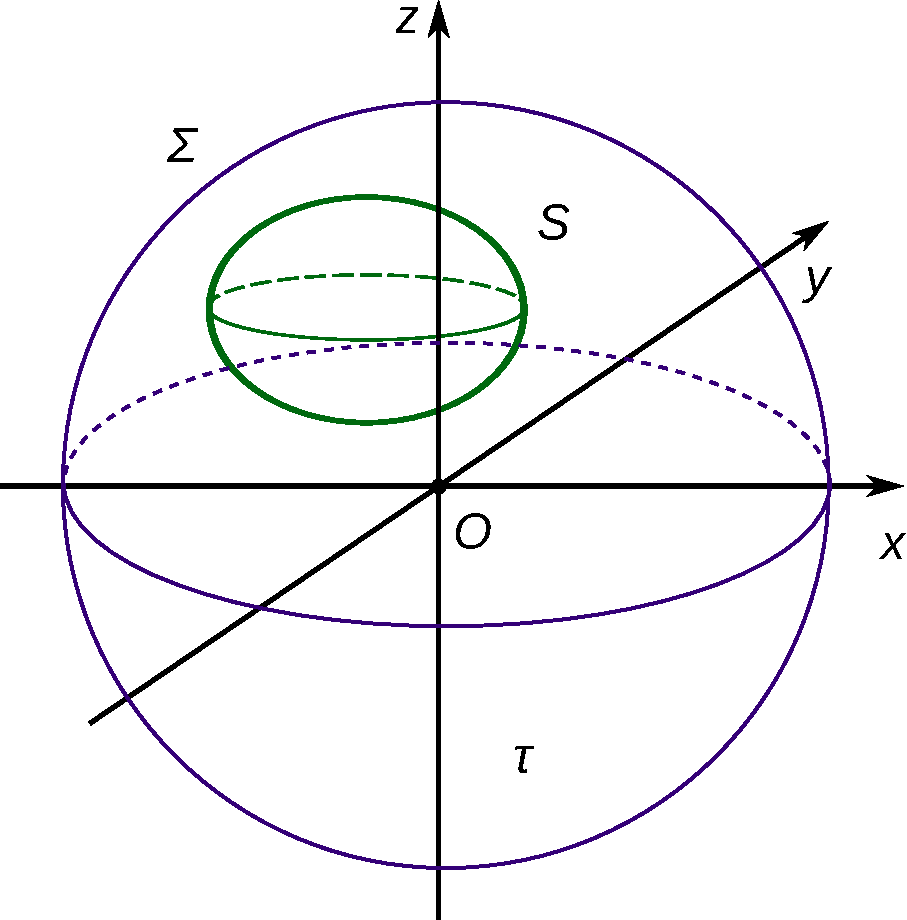
\includegraphics[width=\linewidth]{../img/Sigma_def}
	\end{column}
\end{columns}



}

\frame{
	\frametitle{  Соображения для связи реакции и потенциала }
	
	\begin{exampleblock}{Закон сохранения импульса для объёма $\tau$}
		\parbox{\textwidth}{
		Изменение импульса объёма $\tau$ равно работе сил давления на границах $S$, $\Sigma$ и потери импульса через границу $\Sigma$ результате конвекции:
		\[
		\od{}{t} \int\limits_\tau \rho\vec{v} dV = -\int\limits_{S \cup \Sigma} p\vec{n} dS + \int\limits_\Sigma \rho \vec{v} v_n dS.
		\]
			
		}
	\end{exampleblock}

}

\frame{
	\frametitle{  Соображения для связи реакции и потенциала }
	
	\begin{exampleblock}{Обозначения}
		\parbox{\textwidth}{
			
			Обозначим искомую силу, действующую на тело,
			\[
				\vec{R} = -\int\limits_{S} p\vec{n} dS,
			\]
			Тогда
			\[
			\vec{R} = \od{}{t} \int\limits_\tau \rho\vec{v} dV + \int\limits_{\Sigma} p\vec{n} dS - \int\limits_\Sigma \rho \vec{v} v_n dS =
			\]
			\[
			=
			\rho \od{}{t}\int\limits_\tau \nabla\varphi dV +  
			\int\limits_{\Sigma} \left(
			p\vec{n} - \rho\vec{v}v_n
			\right) dS = 
			\]
			
			
%			Изменение импульса объёма $\tau$ равно работе сил давления на границах $S$, $\Sigma$ и потери импульса через границу $\Sigma$ результате конвекции:
%			\[
%			\od{}{t} \int\limits_\tau \rho\vec{v} dV = -\int\limits_{S \cup \Sigma} p\vec{n} dS + \int\limits_\Sigma \rho \vec{v} v_n dS.
%			\]
			
		}
	\end{exampleblock}
	
}

\frame{
	\frametitle{ Соображения для связи реакции и потенциала }
	\parbox{\textwidth}{
	По теореме Гаусса первый интеграл преобразуется в сумму интегралов по $\Sigma$ и $S$, а во второй подставляем значение для $p$ из интеграла Коши
	\[
	=
	\od{}{t}\int\limits_\Sigma\rho\varphi\vec{n} dS + \od{}{t}\int\limits_S\rho\varphi\vec{n} dS+
	\int\limits_{\Sigma}\left(
	(p_0 - \rho\pd{\varphi}{t} - \frac{\rho v^2}{2})\cdot\vec{n} - \rho\vec{v}v_n
	\right)dS=
	\]\pause
		Так как	поверхность $\Sigma$  не зависит от времени $t$, то
	\[
	\od{}{t}\int_\Sigma\rho\varphi\vec{n}dS = \int_\Sigma\rho\pd{\varphi}{t}\vec{n}dS
	\]
	и, продолжая цепочку,
	\[
	=
	\od{}{t}\int_S\rho\varphi\vec{n} dS + 
	\int_{\Sigma}\left(
	(p_0 - \frac{\rho v^2}{2})\cdot\vec{n} - \rho\vec{v}v_n
	\right)dS=
	\]
	}
	
}

\frame{
	\frametitle{ Соображения для связи реакции и потенциала }
	\parbox{\textwidth}{
	Используя, то что
	\[
	\int_{\Sigma} p_0 \vec{n} dS =  p_0 \int_{\Sigma} \vec{n} dS = 0,
	\]	
	получим продолжение цепочки,
	\[
	=
	\od{}{t}\int_S\rho\varphi\vec{n} dS - \rho
	\int_{\Sigma}\left(
	\frac{ v^2}{2}\vec{n} + \vec{v}v_n
	\right)dS.
	\]\pause
	
	Если положить, что $\Sigma$ -- поверхность сферы радиуса $a$, и вспомнить, что скорость  $v$ стремится к $0$ на бесконечности как $1/a^3$, тогда второе слагаемое в последнем равенстве имеет порядок 
	\[
	 a^2 / (a^3 \cdot a^3) = 1/a^4 \overset{a\to\infty}{\to} 0.
	\]
	}
	
	
	
}

\frame{
	\frametitle{ Связь силы и потенциала  }
	
	\begin{exampleblock}{Выражение для силы}
		\parbox{\textwidth}{
		Сила давлений, действующая на тело в безграничной идеальной жидкости, покоящейся на бесконечности имеет вид
		\[
			\vec{R} = \od{}{t}\int\limits_S\rho\varphi\vec{n} dS.
		\]
		}
	\end{exampleblock}
	
}

\frame{
	\frametitle{ Связь момента сил и потенциала  }
	
	\begin{exampleblock}{Выражение для момента импульса}
		\parbox{\textwidth}{
			Аналогично, записав уравнение сохранения момента импульса для объёма $\tau$, можно получить момент сил давления $\vec{L}$, действующий на тело в безграничной идеальной жидкости, покоящейся на бесконечности
			\[
			\vec{L} = \od{}{t}\int\limits_S\rho\varphi(\vec{r}\times\vec{n}) dS.
			\]
		}
	\end{exampleblock}
	
}

\frame{
	\frametitle{Уравнения движения тела в потоке идеальной жидкости}
	
		\parbox{\textwidth}{
			\[
			\od{\vec{G}}{t} = \od{}{t}\int\limits_S\rho\varphi\vec{n} dS + \vec{F},\quad
			\od{\vec{Q}}{t} = \od{}{t}\int\limits_S\rho\varphi(\vec{r}\times\vec{n}) dS + \vec{M}.
			\]
			\[
			\Downarrow
			\]
			\[
			\od{}{t}\left(
			\vec{G}- \int\limits_S\rho\varphi\vec{n} dS
			\right) =  \vec{F},\quad
			\od{}{t}\left(
			\vec{Q} - \int\limits_S\rho\varphi(\vec{r}\times\vec{n}) dS
			\right) = \vec{M}.
			\]
			
			\medskip
			Здесь $\vec{G}$, $\vec{Q}$ -- собственные импульс и момент импульса тела; $\vec{F}$, $\vec{M}$ -- внешняя сила и момент внешних сил, не связанных движением жидкости. 
		}
	
}

\frame{
	\frametitle{ Уравнения движения тела в потоке идеальной жидкости}
	
	\parbox{\textwidth}{
	Пусть
	\[
	\vec{B} = -\rho\int\limits_S\varphi\vec{n} dS,\quad
	\vec{I} = - \int\limits_S\rho\varphi(\vec{r}\times\vec{n}) dS,
	\]
	тогда уравнения движения принимают вид
	\[
	\od{(\vec{G}+\vec{B})}{t} = \vec{F},\quad
	\od{(\vec{Q}+\vec{I})}{t} = \vec{M},
	\]
	где $\vec{G}+\vec{B}$ называется \alert{импульсивной силой}, а $\vec{Q}+\vec{I}$ -- \alert{импульсивной парой}.
	}
	
}

\frame{
	\frametitle{ Коэффициенты $U_i$  }
	
	\begin{exampleblock}{Новые обозначения}
		\parbox{\textwidth}{
			\[
				U_x = U_1,\quad
				U_y = U_2,\quad
				U_z = U_3,	
			\]
			\[
				\omega_x = U_4,\quad
				\omega_y = U_5,\quad
				\omega_z = U_6.
			\]
			
		}
	\end{exampleblock}

	\begin{exampleblock}{Вид потенциала}
		\parbox{\textwidth}{
			\[
			\varphi = \sum\limits_{k=1}^6U_k \varphi_k.
			\]
		}
	\end{exampleblock}
	
}

\frame{
	\frametitle{ Коэффициенты $B_i$ }
	
	\begin{exampleblock}{Новые обозначения}
		\parbox{\textwidth}{
			\[
				B_x = B_1,\quad
				B_y = B_2,\quad
				B_z = B_3,\quad
				I_x = B_4,\quad
				I_y = B_5,\quad
				I_z = B_6.
			\]
		}
	\end{exampleblock}
	\begin{exampleblock}{Выражения для $B_i$}
		\parbox{\textwidth}{
		\only<1>{
		\[
		B_1 = -\rho\int\limits_S\varphi\alpha dS= -\rho\int\limits_S\varphi\pd{\varphi_1}{n}dS,
		\]
		\[
		B_2 = -\rho\int\limits_S\varphi\beta dS = -\rho\int\limits_S\varphi\pd{\varphi_2}{n}dS,
		\]
		\[
		B_3 = -\rho\int\limits_S\varphi\gamma dS= -\rho\int\limits_S\varphi\pd{\varphi_3}{n}dS,
		\]
		}
		\only<2>{		
		\[
		B_4 = -\rho\int\limits_S\varphi(y\gamma-z\beta) dS = -\rho\int\limits_S\varphi\pd{\varphi_4}{n}dS,
		\]
		\[
		B_5 = -\rho\int\limits_S\varphi(z\alpha-x\gamma) dS = -\rho\int\limits_S\varphi\pd{\varphi_5}{n}dS,
		\]
		\[
		B_6 = -\rho\int\limits_S\varphi(x\beta-y\alpha) dS = -\rho\int\limits_S\varphi\pd{\varphi_6}{n}dS.
		\]
		}
		\only<3>{
		Или в общем виде
		\[
			B_i = -\rho\int\limits_S\varphi\pd{\varphi_i}{n}dS\quad
			(i=\overline{1,6}).
		\]
		}
			
		}
	\end{exampleblock}
}

\frame{
	\frametitle{ Коэффициенты присоединённой массы }
	
	\begin{exampleblock}{Определение}
		\parbox{\textwidth}{
			Подставим выражение для потенциала через переменные $U_i$ в полученное выражение для коэффициентов $B_i$
			\[
			B_i = -\sum\limits_{k=1}^6 \rho U_k \int\limits_S \varphi_k\pd{\varphi_i}{n} dS = \sum\limits_{k=1}^6 \lambda_{ik}U_k, 
			\]
			где
			\[
				\lambda_{ik} = -\rho \int\limits_S \varphi_k\pd{\varphi_i}{n} dS\quad
				(i,k = \overline{1,6}).
			\]\pause
			
			\medskip
			Коэффициенты $\lambda_{ik}$ определяются только геометрией тела и называются \alert{коэффициентами присоединённой массы}.
		}
	\end{exampleblock}
}

\frame{
	\frametitle{Свойства коэффициентов присоединённых масс}
	
	\begin{exampleblock}{Формула Грина}
		\parbox{\textwidth}{
		Для введённого объёма жидкости $\tau$, заключенного между поверхностью сферы большого радиуса $\Sigma$ и поверхностью тела $S$ справедливо равенство
{ \small
		\[
		\int\limits_\tau(\varphi_i\Delta\varphi_k - \varphi_k\Delta\varphi_i)dV 
		=
		\int\limits_\Sigma\left(
		\varphi_i\pd{\varphi_k}{n}-\varphi_k\pd{\varphi_i}{n}
		\right)	dS +
		\int\limits_S\left(
		\varphi_k\pd{\varphi_i}{n}-\varphi_i\pd{\varphi_k}{n}
		\right)	dS.
		\]
}

		}
	\end{exampleblock} \pause
	\begin{exampleblock}{}
		\parbox{\textwidth}{
			
			\only<2>{
			
			В следствии гармоничности $\varphi_i$:
			\[
				\Delta\varphi_i = 0\quad (i=\overline{1,6})
			\]
			левая часть равенства равна $0$. 
			}
			
			\only<3>{
			Интеграл по $\Sigma$ стремиться к $0$ при возрастании радиуса сферы c  одноимённой поверхностью, т.к. площадь сферы имеет порядок $4\pi a^2$, а функции $\varphi_i$ и $\displaystyle\pd{\varphi_k}{n}$ -- $1/a^2$ и $1/a^3$, где $a$ -- радиус сферы.
			}
		
			\only<4>{
			Таким образом, в нашем случае,
			\[
			\int\limits_S \varphi_k\pd{\varphi_i}{n} dS  = 
			\int\limits_S\varphi_i\pd{\varphi_k}{n} dS\quad \Rightarrow \quad
			\lambda_{ik} = \lambda_{ki}\quad (i,k=\overline{1,6}).
			\]
			
			}
		}
	\end{exampleblock}

	
	
}

\frame{
	\frametitle{ Свойства коэффициентов присоединённых масс}
	
	\begin{exampleblock}{Симметричность}
		\parbox{\textwidth}{
		Всего существует $36$ коэффициентов присоединённых масс, но в силу симметрии
		\[
		\lambda_{ik} = \lambda_{ki} \quad (i,k=\overline{1,6}, \, i\neq k)
		\]
		различных всего $21$.
		}
	\end{exampleblock}
}

\frame{
	\frametitle{Кинетическая энергия жидкости}
	
	\begin{exampleblock}{Определение}
		\parbox{\textwidth}{
			Кинетическая энергия объёма $\tau$, ограниченного сферой большого радиуса  $a$ с поверхностью $\Sigma$ и поверхностью тела $S$
			\[
			T_\tau = \frac{\rho}{2}\int\limits_\tau v^2 dV = 
%			\]
%			\[
%			=
			 \frac{\rho}{2}\int\limits_\tau \left[
			 \left( \pd{\varphi}{x} \right)^2 +
 			 \left( \pd{\varphi}{y} \right)^2 +
 			 \left( \pd{\varphi}{y} \right)^2
			 \right]  dV =
			\]\pause
			По формуле Грина
			\[
			=
			 \frac{\rho}{2}\int\limits_\Sigma \varphi\pd{\varphi}{n} dS -  \frac{\rho}{2}\int\limits_S \varphi\pd{\varphi}{n} dS \overset{a \to \infty}{\to}
			-  \frac{\rho}{2}\int\limits_S \varphi\pd{\varphi}{n} dS,
			\]
			т.к. площадь сферы имеет порядок \alert{$4\pi a^2$}, а функции $\varphi$ и $\displaystyle\pd{\varphi}{n}$ --  \alert{$1/a^2$} и \alert{$1/a^3$}.
		}
	\end{exampleblock}
	
}

\frame{
	\frametitle{Кинетическая энергия жидкости}
	
	\begin{exampleblock}{Определение}
		\parbox{\textwidth}{
			Кинетическая энергия всей жидкости
			\[
			T = -\frac{\rho}{2}\int\limits_S \varphi\pd{\varphi}{n} dS.
			\]
			
			Подставляя выражение для разложения Кирхгофа потенциала $\vaphi$
			\[
			T = \frac{1}{2}\sum\limits_{i,k=1}^6 \lambda_{ik} U_k U_i.
			\]
		
		}
	\end{exampleblock}
	
}

\frame{
	\frametitle{ Литература }
	\begin{itemize}[partopsep=1pt,label=\textbullet]
		\item 
		{\em Кочин~Н.~Е., Кибель~И.~А., Розе~Н.~В.} Теоретическая гидромеханика. М.:Гос. издат. физ.-мат. лит., 1963.
		\item {\em Валландер~С.~В.} Лекции по аэрогидромеханике. Учеб. пособие. Л., Изд-во Ленингр. ун-та, 1978. 
	\end{itemize}
}

\end{document}